%\documentclass[a5paper, 10pt]{article}
\documentclass[a4paper, twoside,%landscape, twocolumn, 
12pt]{article}
\usepackage{a4wide}
\usepackage[utf8]{inputenc}
\usepackage[T1]{fontenc}
\usepackage{amsmath}
\usepackage{graphicx}
\usepackage{mathrsfs}
\usepackage{color}
\usepackage{amsmath}
\usepackage{amsfonts}
\usepackage{subcaption}
\usepackage{cmap}
\usepackage{hyperref}
\usepackage[left=2.5cm, right=1.5cm, top=1.5cm, bottom=2cm]{geometry}
\usepackage[czech]{babel} %
\newcommand{\cotg}{\mathrm{cotg}}
\newcommand{\cotgh}{\mathrm{cotgh}}
\newcommand{\tg}{\mathrm{tg}}
\newcommand{\tgh}{\mathrm{tgh}}
\newcommand{\Ci}{\mathrm{Ci}}
\newcommand{\Si}{\mathrm{Si}}
\newcommand{\Li}{\mathrm{Li}}
\newcommand{\I}{\mathrm{i}}
\newcommand{\dif}{\mathrm{d}}
\newcommand{\R}{\mathbb{R}}
\newcommand{\pard}[2]{\frac{\partial #1 }{\partial #2 }}
\newcommand{\der}[2]{\frac{\mathrm{d} #1 }{\mathrm{d} #2 }}
\newcommand{\e}{\mathrm{e}}
\newcommand{\V}{\mathbb{V}}
\newcommand{\Z}{\mathbb{Z}}
\newcommand{\N}{\mathbb{N}}
\newcommand{\F}{\mathscr{F}}
\newcommand{\G}{\mathscr{G}}
\newcommand{\Hz}{\mathscr{H}}
\newcommand{\C}{\mathbb{C}}
\newcommand{\Q}{\mathbb{Q}}
\author{Jakub Dokulil}
\newcommand{\A}{\mathscr{A}}
\title{Věty a myšlenky jejich důkazů k mat analýze 2.}
\begin{document}
\begin{table}[h!]
\begin{tabular}{p{0.9\textwidth}}
    \textsf{\huge{Matematická analýza 2 lidsky}}\newline \textsf{\textbf{\Large Jakub Dokulil}}\\
    \hline
\end{tabular}
\end{table}

\noindent\textsf{Vytvořeno pro zjednodušení a lepší interpretaci složitých matematických definic od Lůďy $\heartsuit$. Proto neručím správnost. Poslední aktualizace \today. Šiřte a upravujte podle svého gusta.}

\textsf{
    Před zkouškou\\
    --------------\\
    Podrobněji projít Jordanovu míru!
}

\tableofcontents

\section{Metrické prostory}

Nechápatmnožinu $\R ^n$ pouze jako množinu $n$-tic, ale jako množinu na níž jsou nadefinovány operace sčítání a násobení skalárem - \textbf{vektorový prostor nad $\R$}.

Metrický prostor $M$ s prvky $x,y \in M$ splňuje následující axiomy:
\begin{itemize}
    \item Totožné body jsou od sebe vzdálené 0
    \item vzálenost x od y, je stejná jako vzdálenost y od x (symetrie)
    \item platí trojúhelníková nerovnost $|xy|\leq |xy| + |yz| $ ($\rho(x,y)\leq \rho(x,y) + \rho(y,z) $)
\end{itemize}
\textbf{Metrika na $M$} = Vzdálenost bodů je nadefinována jako zobrazení $\rho: M\times M \rightarrow \R^+$

\paragraph{Metrický prostor} je dvojce $(M, \rho)$
\begin{description}
    \item[Druhy metrik] \begin{description}
        \item[Manhattanská] - pravoúhlý systém, $|x_1 - y_1|+|x_2 - y_2|+ \dots +|x_n - y_n|$
        \item[Eukleidovská] - nejkratší možná cesta $\sqrt{(x_1 - y_1)^2 + (x_2 - y_2)^2 + \cdots }$ 
        \item[Šachovnicová] - nejvzdálenější souřadnice $\max\{ |x_1 - y_1|,\,|x_2 - y_2|,\, \dots,\,|x_n - y_n| \}$
    \end{description} 
    \item[Koule a okolí] --    
    \begin{description}
        \item[Koule] je množina bodů $X$ metrického prostoru $(M, \rho)$, které mají od jejího středu $a$ stejnou \uv{vzdálenost} ($\rho(a,X)= $ konst.) 
        \item[Ryzí okolí] bodu $a$ je koule bez středu.
    \end{description}
    \item[Vzdálenst prostorů, průměr] --
    \begin{description}
        \item[vzdálenost] množin $\rho (A,B)$ v metr. prostoru, je jejich nekratší spojnice -- $\inf\lbrace \rho(a,b); a \in A; b \in B \rbrace$
        \item[průměr] množiny $d(A)$ je nevětší vzdálenost dvou prvků množiny, $\sup\lbrace \dots$
    \end{description}
\end{description}

\begin{figure}[h]
    \centering
    \begin{subfigure}[b]{10cm}
        \input{vzd_mnozin.pdf_tex}
        \caption{}
    \end{subfigure}
    \begin{subfigure}[b]{0.3\textwidth}
        \input{prum_mnoziny.pdf_tex}
        \caption{}
    \end{subfigure}
    %\def\svgwidth{10cm}
    \caption{(a) vzdálenost množin. (b) Průměr množiny.}
    \label{}
\end{figure}

\section{Podmnožiny metrickém prostoru}
\begin{description}
    \item[Pojmy:] spojené s množinou $A$ v metrickém prostoru. 
    \begin{description}
        \item[vnitřní bod] -- alespoň jedno okolí bodu je součástí množiny (\textbf{vnitřek -- $A^\circ$})
        \item[hraniční bod] -- \emph{není ani v množině ani mimo ni}. Jeho okolí má prázdný průnik s množinou ($O(a)\cap A = \emptyset$), ale i se zbytkem prostoru ($ O(a)\cap (M\backslash A) = \emptyset$) (\textbf{hranice -- $\partial A$})
        \item[bod uzávěru] vzdálenost od množiny je 0 (\textbf{uzávěr -- $\bar{A}$})
        \item[hrom. bod] - každé okolí není prázdné (\textbf{hrom body -- $ A'$})
        \item[izolovaný bod] - existuje okolí, ve kterém je bod sám   
    \end{description}
    \item[otevřená množina] pro množina je svým vnitřkem, nemá hranici
    \item[uzavřená množina] každý bod má nulovou vzdálenost od ní, je sama svým užávěrem
\end{description}
\section{Konvergence v metrickém prostoru}
Polsoupnost bodů $\lbrace x_n \rbrace$ si lze představit jako diskrétně rozložené body v metrickém prostoru (například body v rovině).
\begin{description}
    \item[Konvergentní posloupnost] -- vzdálenost (metrika) bodů konverguje k nule. Posloupnost $x_n$ konverguje k bodu $x$ pokud se k bodu podle metriky blíží -- $\lim_{n\to\inf} \rho(x_n, x) = 0$
    \item[Ohraničená posloupnost] - pokud množina výsledků posloupnosti, funkčních hodnot, je ohraničená. (má konečný průměr)
    \item[Cauchyovská] - od určitého $n_0$ leží každé dvě funkční hodnoty v $\varepsilon$ okolí.
    $$ \text{konvergentní} \Rightarrow \text{Cauchyovská}$$ 
    \emph{Důkaz věty} -- zvolit $\frac{\varepsilon}{2}$ a použít trojúhelníkovou nerovnost.
    \item[Uzavřenost a konvergence] -- podmnožina metrického prostoru $A$ je uzavřená $\Leftrightarrow$ každá konvergentní posloupnost v podmnožině konverguje k $a$ posloupnost konvergující k $a\in A$ 
    \item[Uzavřenost a konvergence] -- podmnožina metrického prostoru $A$ je uzavřená $\Leftrightarrow$ každá konvergentní posloupnost v podmnožině konverguje k $a$, pak $a\in A$ 
    \item[ekv metriky] metriky jsou ekvivalentní pokud konvergentní posloupnosti dávají stejnou konvergenci
    \item[ekv metriky jinak] metriky $\rho, \sigma$ jsou ekvivalentní pokud existují kladná čísla $a, b$ tak, aby
    $$ a\sigma \leq \rho \leq b\sigma $$
    \emph{Důkaz:} vezme se konvergentní posloupnost bodů $x_n$ tak aby $\lim \sigma (x_n, a) = 0$ s využitím věty o třech posloupnostech platí $\lim \rho (x_n, a) = 0$.
    \item[indukované metriky] podprostor metrického prostoru má svou vlastní metriku shodnou s tou originální (například aplikace metriky pro $\R^2$ na $\R$, kde se uvažuj, že prvky $a$ z $\R$ lze zapsat jako $(a,0)$.
\end{description}

\section{Úplné a kompaktní metrické prostory}
V úplném prostoru má každá Cauchyovská posloupnost má limitu náležící danému prostoru. ({Například} $\Q$ s Eukleidovskou metrikou, posloupnost $\left\lbrace\frac{1}{n}+n\right\rbrace$ konverguje k $\e \notin \Q$ ).
\begin{description}
    %\begin{itemize}
        \item[] uzavřená podmnožina úplného prostoru je úplná.
        \item[Kompaktní prostor] -- ze všech posloupností jeho bodů, které obsahuje lze vybrat konvergentní posloupnost
        $$ A \text{ kompaktní množina v prostoru} \Rightarrow A \text{ uzavřená a ohraničená} $$
        $A$ je uzavřený a ačkoli může mít díru nesmí se jednat o pěnu.\\
        \emph{Pozn1:} Pro prostory $(\R^n, \rho_i),\, i = 1,2, \infty$ platí implikace ( kompaktní $\Leftrightarrow$ uzavřená a ohraničená)\\
        \emph{Pozn2:} Kompakní prostor je vždy úplný.
    %\end{itemize}
\end{description}
\section{Zobrazení}
\begin{description}
    \item[Izometrické zobr.] takové které zachovává vzdálenost ($F: (M, \rho)\rightarrow(N, \sigma)$ pak  $\rho(x,y)=\sigma(F(x), F(y))$.)
    \item[Spojité zobrazení] $x$ z $\varepsilon$-okolí se zobrazí na $F(x)$ z $\delta$-okolí $F(x_0)$.
    \item[Heineho podm.] pokud $x$ konverguje k $x_0$ pak $F(x)$ konverguje k $x_0$.
    \item[zobrazení kompaktní mn] kompaktní množina se zobrazí na kompaktní množinu. (Důsledkem jsou Weierstrassovy věty.)
    \item[Stejnoměrně spojité zobrazení] dvojce vzor obraz lze projet $\varepsilon-\delta$-okoím ($\rho(x,y)<\delta$, $\sigma(F(x),F(y))<\varepsilon$)
    \item[Heine-Cantor]\footnote{\emph{Pro $\R$:} je-li funkce spojitá na intervalu $\left< a,\,b\right>$, pak je na něm také stejnoměrně spojitá.} -- prostor $M$ je kompaktní, zobr. $F$ je spojité, pak $F$ je stejnoměrně spojité.
    \item[Lipschitzovské zobrazení] Lineárně násobí (škáluje) vzdálenosti. Existuje $L>0$ tak, že $\sigma(F(x),F(y)) = L \rho(x,y)$ (vzdálenost obrazů dvou bodů je menší jak násobek vzdálenosti bodů samotných.)
    $$\text{Lipschitzovské} \Rightarrow \text{Stejnoměrně spojité}$$
    \textbf{Kontrakce} je zobrazení s $0<L<1$ 
    \item[Limita zobrazení] $x_0$ je hromadný bod množiny $M$, zobrazení v něm má limitu\footnote{\textbf{Pozor:} od Nechvátalových materiálů se liší značení. V materiálech je značena $y_0$ nikoli $a$. } $a$ jestliže $x$ z ryzího $\delta$ okolí ($x \in O_\delta^* (x_0)$) se zobrazí do $\varepsilon$-okolí $a$ ($F(x)\in O_\varepsilon ^* (x_0)$)
    \item[Pevný bod] se zobrazí sám na sebe ($F: M\rightarrow M, F(x)=x$) 
    \item[Banachova věta] o pevném bodu. Pokud je zobrazení kontrakcí, pak existuje jediný pevný bod.
\end{description}

\section{Funkce $n$ proměnných}

Funkce n proměnných je zadefinována jako zobrazení 
$$ f:\: \R^n \rightarrow \R. $$
\begin{description}
    \item[Def. obor] množina $x\in\R^n$ tak, že k němu existuje obraz.
    \item[Obor hodnot] množina $y\in\R$, tak že je obrazem nějakého $x$.
    \item \emph{pozn:} Spojitost zevdena podle předchozí kapitoly. Zavadí se \uv{nelastní případ} $(\R^*)^n = \underbrace{\R^* \times \R^* \times \dots \times \R^*}_{n\text{-krát}}$. Pro okolí se používá šachovnicová metrika $\rho_\infty$.
    \item[Limita funkce] funkce má v bodě $a$ limitu pokud se $x$ z ryzího $\delta$-okolí zobrazí do $\varepsilon$-okolí.
    \item[věta 6.7] funkce má v bodě limitu pokud se zobrazí na kruhové okolí obrazu
    \item[parciální derivace] definovanéá pomocí limity $h\to 0$ se přičítá jen k jedné proměnné.
    $$\pard{f(x_0, y_0)}{x} =  f_x' (x_0, y_0) = \lim_{h\to 0} \frac{f(x_0+h,y_0) - f(x_0, y_0)}{h} $$
\end{description}

\section{Parciální a směrová derivace}

\begin{description}    
    \item[Schwarzova v.] druhé parciální derivace podle různých proměnných jsou záměnné
    $$ \frac{\partial^2 f(X)}{\partial x_n \partial x_m} = \frac{\partial^2 f(X)}{\partial x_m \partial x_n} $$
    \item[Směrová derivace] definičním oborem se vede přímka nebo rovina v požadovaném směru, která se derivuje.
    $$ \phi(t) = f(x_0 + s_1 t, y_0 + s_2 t)  $$
    \item[Gradient] funkce f
    $$\nabla f = \left( \pard{f}{x_1},\, \pard{f}{x_2}, \,\dots ,\, \pard{f}{x_n}  \right)$$  
\end{description}

\section{Implicitní funkce}

Pokud funkce $F: \R^2 \to \R$ ma nulový bod $[x_0, y_0]$ ($F(x_0, y_0)=0$). V okolí takového bodu je funkce $y=f(x)$ definovaná \emph{implicitně} rovnicí $F(x,y)=0$, pokud na $\delta$-okolí bodu $x_0$ platí $F(x,f(x))=0$. Tedy vybere jen takové body z okolí $x_0$ viz \ref{fig:implic}, které následně budou tvořit funkci $f$.
{\small Zkusit chápat tak, že se nejprve z nulového bodu určí funkce $f$ a následně pomocí této funkce se najdou zbylé body z $\R^2$, které budou tvořit funkci $f$.}

\begin{figure}[]
    \centering
    \input{impl.pdf_tex}
    \caption{okolí nulového bodu pro následnou implicitní funkci.}
    \label{fig:implic}
\end{figure}

\paragraph{Věta o existenci impl. funkce} Implicitní funkce existuje pokud ($\Leftarrow$) 
\begin{enumerate}
    \item $F$ je spojitá na čtverci $R$ ($a$-okolí bodu $x_0,y_0$ v $\rho_\infty$),
    \item existuje $\pard{F}{y}$ spojitá v b. $[x_0, y_0]$,
    \item $\pard{F(x_0, y_0)}{y} \neq 0$ -- viz příklad s kružnicí, pro $x=r$ a $y=0$, pak se nemusí jednat o zobrazení, jednomu $x$ mohou být přiřazena dvě $y$.
\end{enumerate}

\paragraph{Derivace impl funkce}
je definována jako 

$$ \der{f(x_0)}{x} = \frac{\pard{F(x_0, y_0)}{x}}{\pard{F(x_0, y_0)}{y}} $$

Pokud jsou druhé derivace také spojité, tak lze určit druhou derivaci:

\paragraph{impl funkce dvou proměnných}
podobně lze definovat i pro zobrazení $F: \R^3 \to \R$ a $z = f(x,y)$, zde se definuje pro $\delta$ - okolí $(x-\delta, x+\delta)\times (y-\delta, y+\delta)$ bodu $f(x,y,f(x,y))$.

\subparagraph{Derivace}
$$\pard{f(x_0,y_0)}{x} = \frac{\pard{F(x_0,y_0, z_0)}{x}}{\pard{F(x_0,y_0, z_0)}{z}},\qquad \pard{f(x_0,y_0)}{y} = \frac{\pard{F(x_0,y_0, z_0)}{y}}{\pard{F(x_0,y_0, z_0)}{z}} $$

\begin{figure}[h]
    \centering
    \begin{subfigure}[b]{7cm}
        \input{okoli1.pdf_tex}
        \caption{}
    \end{subfigure}
    \begin{subfigure}[b]{7cm}
        \input{okoli2.pdf_tex}
        \caption{}
    \end{subfigure}
    \begin{subfigure}[b]{7cm}
        \input{okoli3.pdf_tex}
        \caption{}
    \end{subfigure}
    %\def\svgwidth{10cm}
    \caption{(a)  (b) (c) }
    \label{}
\end{figure}

\paragraph{$m$-funkce} zjednodušeně $\F : \R^n \to R^m $. Přesněji:
$$\F: [x_1, x_2, \dots, x_n] \to [f_1(x_1, x_2, \dots, x_n), f_2(x_1, x_2, \dots, x_n), \dots, f_m(x_1, x_2, \dots, x_n)] $$
čili $\F$ vektor $\to$ vektor, proto se také někdy mluví o \emph{vektorovém poli}.

\subparagraph{Diferencovatelnost}
Funkce $\F$ je difencovatelná pokud všechny funkce  $f_1$ až $f_m$ jsou diferencovatelné. Pak
$$\dif\F(X_0): [h_1, h_2, \dots h_n] \to [\dif f_1(X_O), \dif f_2(X_0), \dots, \dif f_m(X_0)]$$
lze jej také určit Jacobiovou maticí $\F'$ (maticí prvních derivací)
$$ \F' = \left(\begin{array}{cccc}
    \pard{f_1}{x_1}&\pard{f_1}{x_2}& \cdots &\pard{f_1}{x_n}\\
    \pard{f_2}{x_1}&\pard{f_2}{x_2}& \cdots &\pard{f_2}{x_n}\\
    \vdots&\vdots&  & \vdots\\
    \pard{f_m}{x_1}&\pard{f_m}{x_2}& \cdots &\pard{f_m}{x_n}\\
\end{array} \right) $$
a pak totální diferenciíl je:
$$\left(\begin{array}{c}
    \dif f_1 (X_0)\\
    \dif f_2 (X_0)\\
    \vdots\\
    \dif f_m (X_0)\\
\end{array} \right) = \F' (X_0) \left( \begin{array}{c}
    \dif h_1 \\
    \dif h_2 \\
    \vdots\\
    \dif h_n \\
\end{array}
\right) $$
$\F' (X_0)$ je zde matice hodnot prvních derivací.

Pro $m=n$ se determinant Jacobiho matice nazývá \emph{Jacobián}. a značí se $J_\F (X_0)$

\subparagraph{Matice složeného zobrazení:} Jacobiho matice složeného zobrazení $\Hz = \F \circ \G$ je součinem matic jednotlivých zobrazení $\Hz' (X_0) = \F'(Y_0) \G'(X_0)$. Pokud máme zobrazení $\G : R^n \to \R^m $ a $\F : R^m \to R^p$ a zobrazení 

\subparagraph{Lokální inverze} Pokud je v bodě $\F$ Jacobián nulový, pak je zobrazení v bodě tomto prosté. Pak platí:
% Pokud je v nějakém bodě zobrazení $\R^n \to \R^n$ Jacobián nulový ($J_\F (X_0)=0$) pak na nějakém okolí tohoto bodu $O(X_O)$ je $\F$ prosté. V bodě $Y_0 = \F(X_0)$ platí
$$ (\F^{-1})'(Y_0)=(\F'(X_0))^{-1} \quad a \quad J_{\F^{-1}} = \frac{1}{J_\F (X_0)} $$

\subparagraph{Implicitní $m$-funkce} Pokud je $\G: \R^{n+m}\to \R^m $ 
\begin{itemize}
    \item spojitá na okolí bodu $\left[X_0, Y_0\right] = \left[\underbrace{x^0_1, x^0_2 , \dots, x^0_n}_{n \text{prvků}}, \underbrace{y^0_1, y^0_2, \dots y^0_m}_{m \text{prvků}}\right]$ $O_a ([X_0, Y_0 ])$
    \item a funkce je v bodě nulová, $\G (X_0, Y_0)=(0, 0, \dots, 0)$
    \item a všechny funkce $\G = (g_1, g_2, \dots, g_n)$ jsou derivovatelné podle všech proměnných $y_1, y_2, \dots, y_n$ -- \textsf{aby v okolí nikam zběsile neskákala, ale měnila se předvídatelně, \textbf{zapisuje se do Jacobiho matice!}}
\end{itemize}
pak je implicitně zadána jediná spojitá $m$-funkce 
$$ Y = \F(X) $$

\section{Vázané extrémy}
\paragraph{Vázaný extrém} je extrém z vybrané podmnožiny definičního oboru, přičemž podmnožina bývá definována soustavou rovnic (\emph{podmínky vázaného extrému}). Vázaný extrém $X_0$ funkce $F: \R^n \to \R$ je definován tak, že existuje podokolí na $M$ kde má funkce extrém.

\paragraph{Lagrangeovy multiplikátory} nechť máme funkci $f$ a podmínky $g_1, \dots, g_m$. Dohromady dávají zobrazení $\R^n \to \R$ ($1\leq m<n$) a mají spojité všechny parciální derivace. Nechť Jacobiho matice $\G'$ m-funkce $\G$ má hodnost $m$ (podímnky jsou na sobě nezávislé). Pak je li v $X_0$ vázený extrém platí
$$\pard{f}{x_j} + \sum^{m} \lambda_k \pard{g_k}{x_j} = 0 $$
\textsf{tj pokud se k derivaci podle jedné proměnné přičnou násobky derivací podmínek podle druhé proměnné dostaneme nulu}.

\subparagraph{Stacionární bod} -- bod pro který existují L. multiplikátory, tak že vyhovují podmínce.
Lze je nalézt pomocí Lagrangeovy funkce 
$$ L(x_1, x_2, \dots, x_n, \lambda_1, \lambda_2, \dots, \lambda_m) = f(x_1, x_2, \dots, x_n) + \sum^{m} \lambda_k g_k $$
Položí se $\vec\nabla L = 0$ čímž vzniká vztah výše.

\textbf{Zda-li je v stac bodě $S$ extrém se určí pomocí druhého diferenciálu $\dif^2 L(S, \Lambda_S)$} Pozitivně definitní $\Rightarrow$ minimum.

\section{Dvojný intergrál}

Cílem je nalézt objem pod pochou na obdélníku $I = \left< a,b\right> \times \left<c,d\right>$. 

\begin{enumerate}
    \item Dělení obdélníku $I$ na na $n\times m$ menších obdélníčků $I_{i,j}$. Dělení je značeno $D$. $D_x: a<x_1<x_2<\dots<x_n=b$, $D_y$ -- obdobně 
    \item Obsah obdélníčku $I_{ij}$ je značen $\lambda(I_{ij}) = (x_i - x_{i-1})(y_i - y_{i-1})$
    \item Horní a dolní hodnota 
    \begin{itemize}
        \item $M_{ij}$ - supremum funkce na obdélníčku $ij$
        \item $m_{ij}$ - infimum funkce na obdélníčku $ij$
    \end{itemize}
    \item Horní a dolní součet. Součet \uv{dolního a horního objemu}
    $$s(f,D) = \sum_{i=1}^n \sum_{j=1}^m m_{ij} \lambda(I_ij) \quad S(f,D) = \sum_{i=1}^n \sum_{j=1}^m M_{ij} \lambda(I_ij)$$
    \item Pro všechna dělení $D \in \mathscr{D}$ platí, že dolní a horní intergrál (dolní je největších z těch pod křivkou a horní \dots)
    $$ \iint_{\underline{I}} f(x,y)\dif x\dif y = \sup\lbrace s(D,f): \: D \in \mathscr{D} \rbrace \quad \iint_{\overline{I}} f(x,y)\dif x\dif y = \inf\lbrace S(D,f): \: D \in \mathscr{D} \rbrace $$
    \item Riemanův integrál hodnota integrálů, pokud 
    $$ \iint_{\underline{I}} f(x,y)\dif x\dif y = \iint_{\overline{I}} f(x,y)\dif x\dif y $$
\end{enumerate}

Platí:
$$ \text{Spojitá na obdelníku} \Rightarrow \text{integrovatelná na obdelníku}$$

\paragraph{Fubiniho v.} \emph{Nejdřív jeden rozměr (integrál), pak druhý rozměr}. Pokud máme obdelník $I = \left< a,b\right> \times \left<c,d\right>$, pak integrál lze spočítat jako 
$$ \iint_I f(x,y)\dif x\dif y = \int_a^b \left( \int_c^d f(x,y) \dif y\right) \dif x  $$

\paragraph{Normální množina} Například normání množina vzhledem k ose x znamená, že množina je pro $x\in\left< a,b\right>$ vymezena funkcemi $\varphi_1, \varphi_2$ (funkce se nesmí křížit, tj, $\varphi_1<\varphi_2$). Pak \textbf{Fubiniho věta nabývá obecnější podoby}
$$ \iint_{M_x} f(x,y)\dif x\dif y = \int_a^b \left( \int_{\varphi_1}^{\varphi_2} f(x,y) \dif y\right) \dif x;  \quad \iint_{M_y} f(x,y)\dif x\dif y = \int_c^d \left( \int_{\psi_1}^{\psi_2} f(x,y) \dif x\right) \dif y $$

\begin{figure}[h]
    \centering
    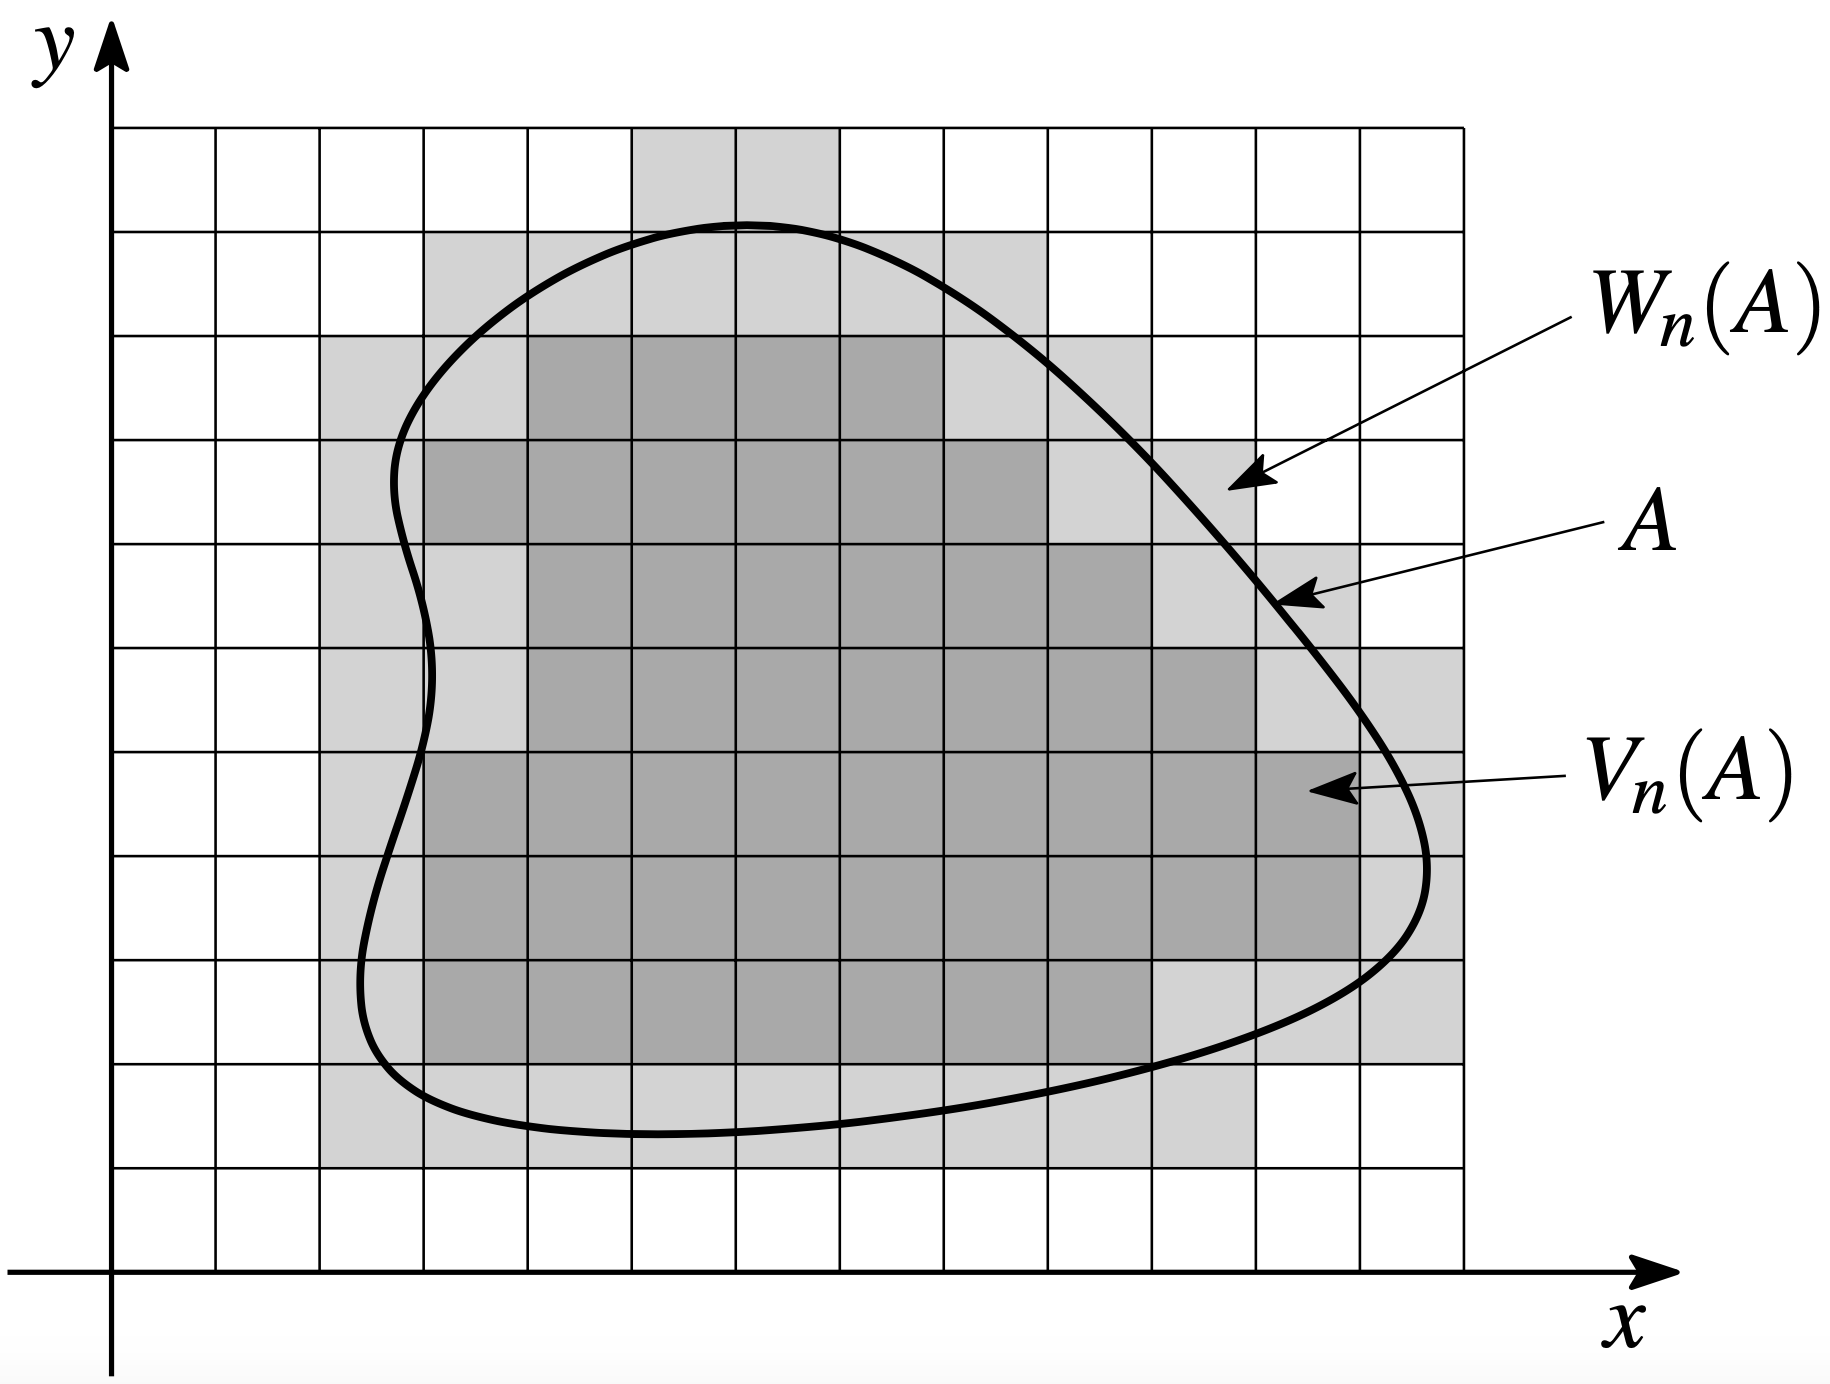
\includegraphics[width=10cm]{jordan_sit.png}
    \caption{Jádro řádu n (tmavší šedá) a obal řádu n (světlejší šedá) množiny A (čtverce jádra jsou zároveň čtverci obalu).}
    \label{fig:jordan}
\end{figure}

\section{Jordanův přístup k dvojnému integrálu}

\paragraph{Míra množiny $\lambda$} je \emph{cosi jako obsah}. Zobrazení $\R^2 \to \R^+$. Měla by splňovat následující podmínky
\begin{itemize}
    \item $A=B\; \rightarrow \; \lambda(A) = \lambda(B)$ - stejná množina, stejný obsah
    \item $A\subseteq B\; \rightarrow \; \lambda(A) \leq \lambda(B)$ menší množina, menší obsah
    \item $A\cap B = \emptyset\; \rightarrow \; \lambda(A\cup B ) \lambda(A) + \lambda(B)$
\end{itemize}

Nadefinuje se síť řádu $n$, kde \emph{čím větší $n$ tím menší čtverečky}. Pak j-tý a k-tý čtverec je brán jako
$$ Q_{j,k}^n = \lbrace [x,y]\in \R^2: \frac{j}{2^n} \leq x \leq \frac{j+1}{2^n}, \frac{k}{2^n} \leq y \leq \frac{k+1}{2^n}\rbrace $$
Jelikož má jeden čtverec stranu $\frac{1}{2^n}$ tak potom jeho míra, \emph{obsah} je:
$$\lambda(Q_{j,k}^n ) = \left(\frac{1}{2^n}\right)^2$$

\end{document}